\documentclass[12pt,a4paper]{report}

%Set language
\usepackage[english]{babel}
\usepackage{enumerate}

% To import and adjust images
\usepackage{graphicx}
\usepackage[export]{adjustbox}
\usepackage[center]{caption}
\usepackage{subcaption}
\usepackage{float}
\usepackage{tabularx}
\usepackage{lipsum}

% To use monospaced font
\usepackage{courier}

% To build a clickable Toc
\usepackage{color} %May be necessary if you want to color links
\usepackage{hyperref}
\hypersetup{
    colorlinks=true, %set true if you want colored links
    linktoc=all,     %set to all if you want both sections and subsections linked
    linkcolor=black,  %choose some color if you want links to stand out
    urlcolor = black
}


%To load PoLitecnico's logo
\usepackage{titling}

% Command to hide subsections in the Toc
\setcounter{tocdepth}{1}

% I don't like dots in the Toc
\usepackage{tocloft}
\renewcommand{\cftdot}{}

%To improve the tables
\usepackage[table]{xcolor}

%To break line inside tables
%\usepackage[utf8]{inputenc}
%\usepackage{fourier} 
%\usepackage{array}
\usepackage{makecell}
%\renewcommand\theadalign{bc}
%\renewcommand\theadfont{\bfseries}
\renewcommand\theadgape{\Gape[4pt]}

% Path relative to the .tex file containing the \includegraphics command
\graphicspath{ {./images/} }

% To change the ToC title
\addto\captionsenglish{ \renewcommand {\contentsname} {Table of contents}}

%logo
\pretitle{
	 \begin{center}
	 \LARGE
	 
\includegraphics[width = 0.6\textwidth]{logo}\\[\bigskipamount]
}
\posttitle{\end{center}}

% Here we go
\title{Data Intelligence Applications Homework}
\author{D'Amato Francesco, \\
	Frantuma Elia - 10567359 - 945729, \\
	Fucci Tiziano - 10524029 - 946638}
\date{A.Y. 2020/2021}

\begin{document}
	\maketitle
	%Index
	\tableofcontents
	\chapter{Introduction}
		\section{Scenario}
			Consider the scenario in which advertisement is used to attract users on an ecommerce website and the users, after the purchase of the first unit of a consumable item, will buy additional units of the same item in future. The goal is to find the best joint bidding and pricing strategy taking into account future purchases.

\begin{figure}[H]
\centering
  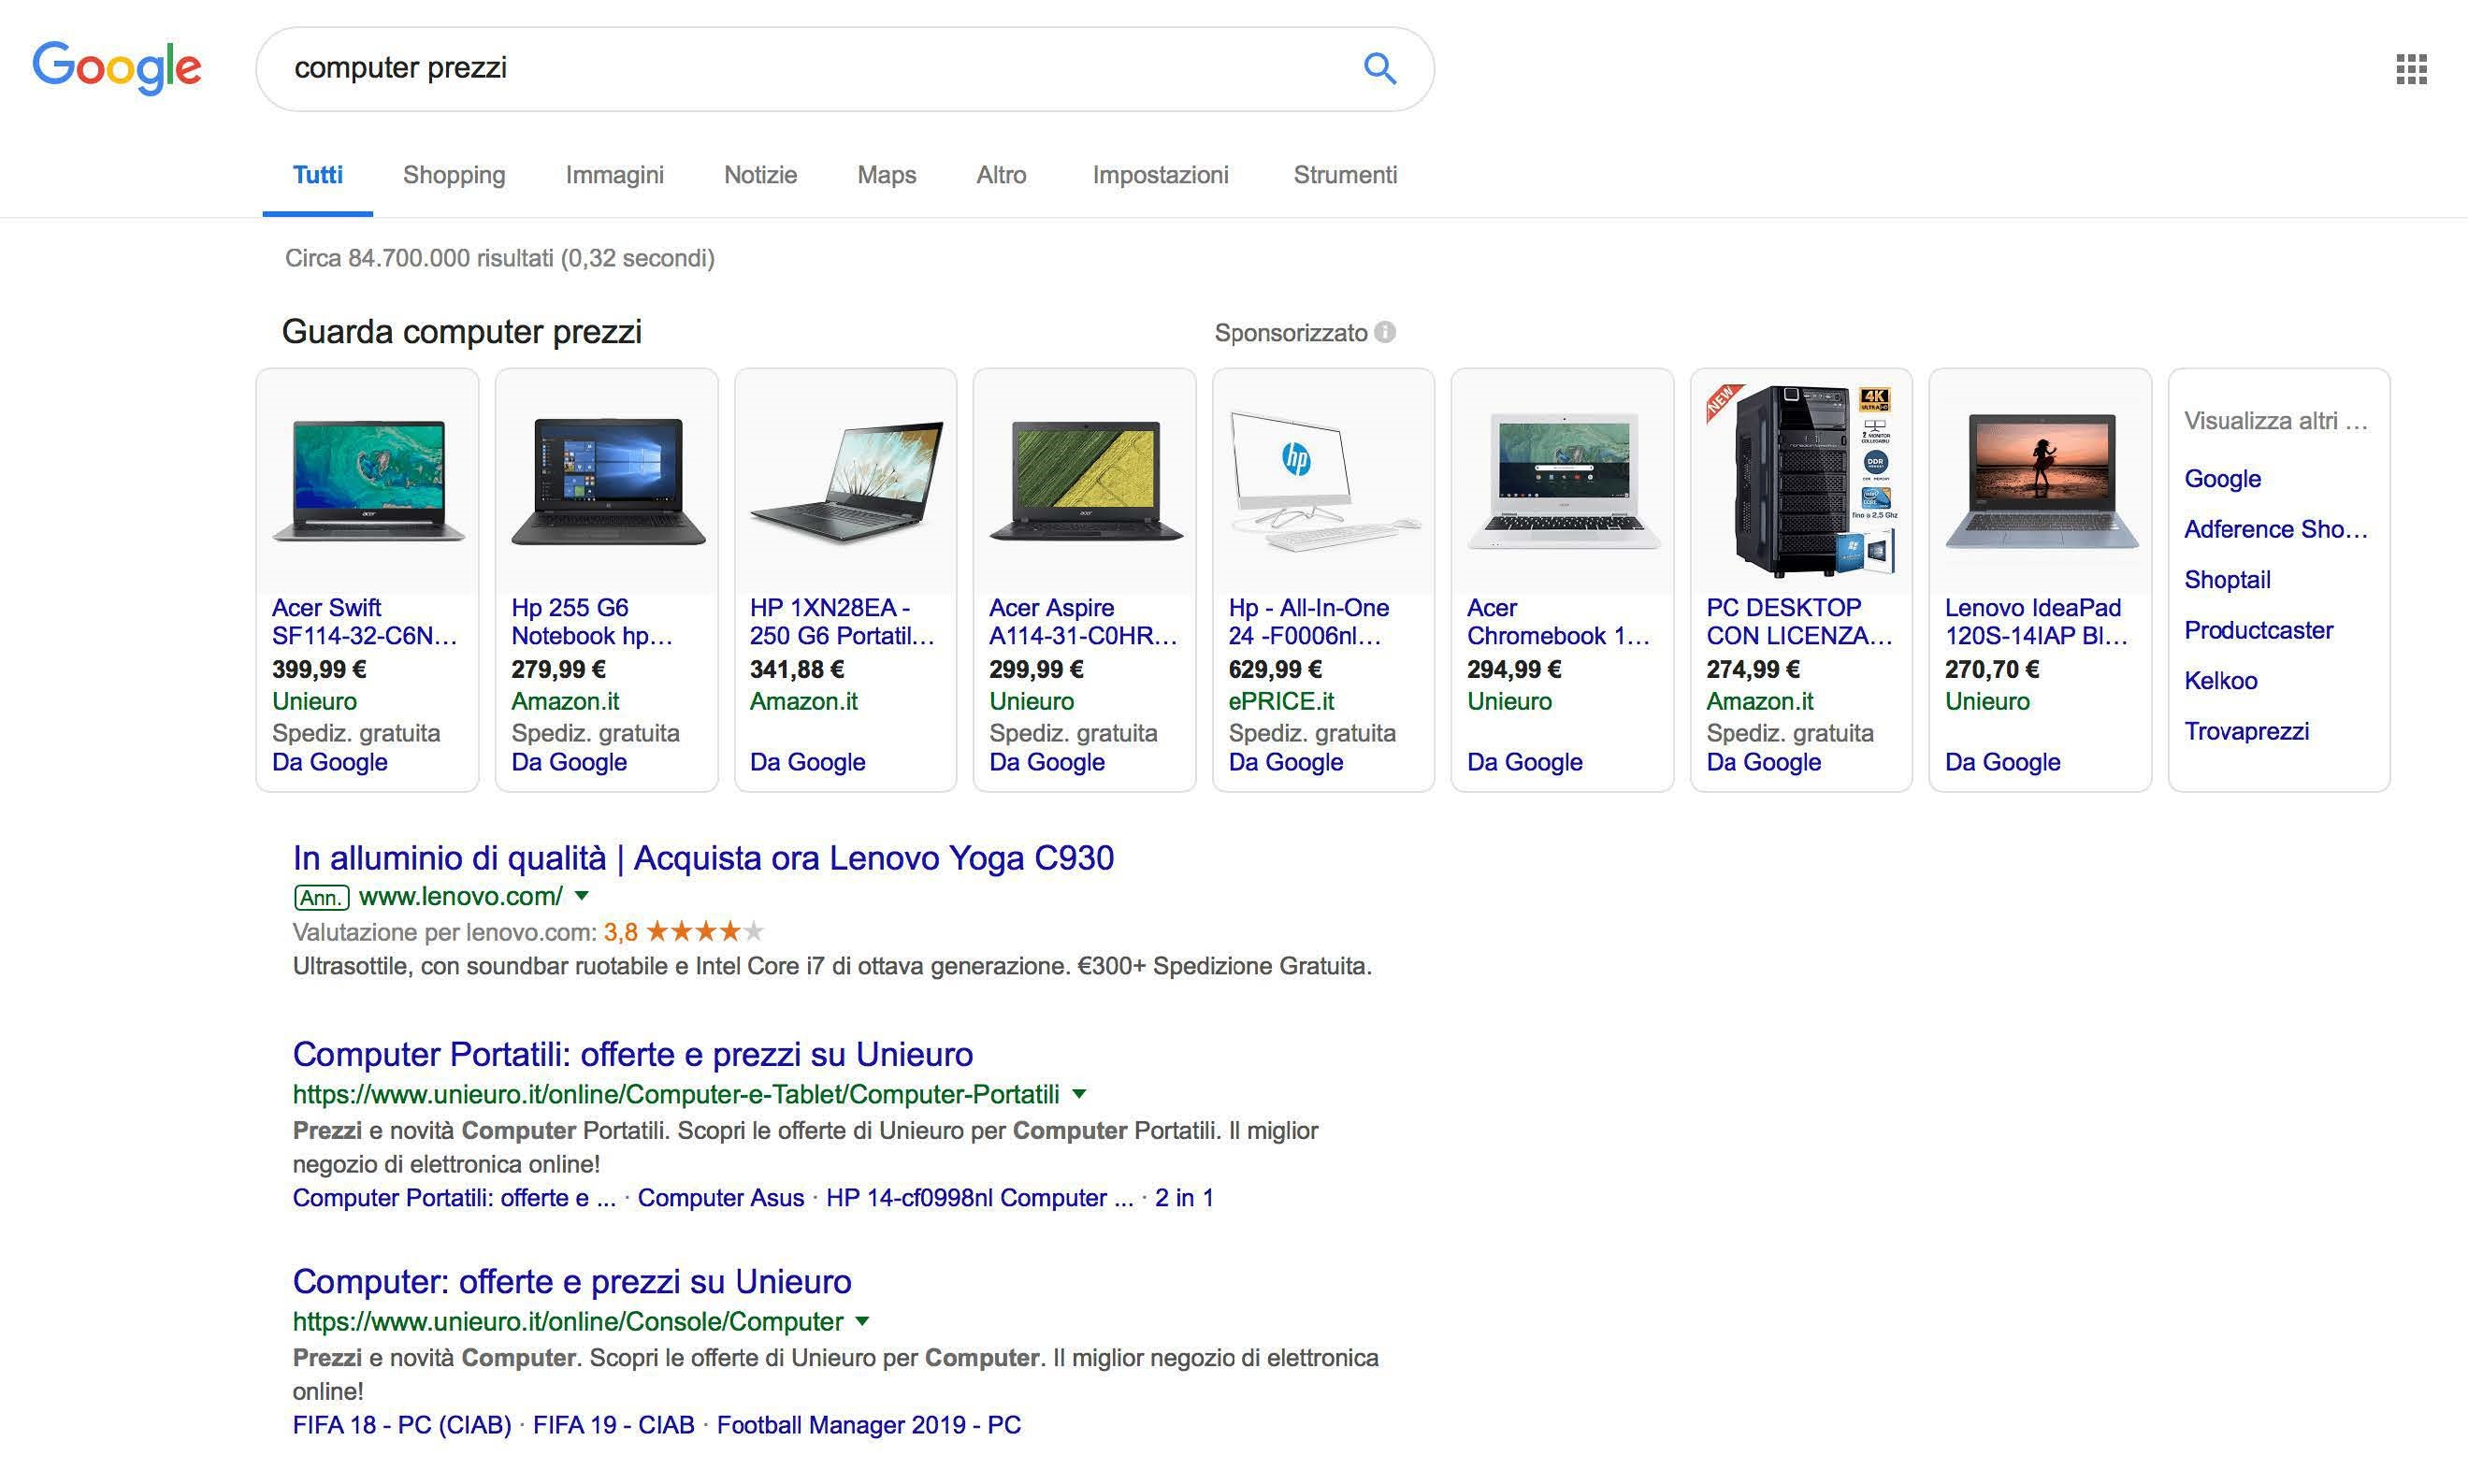
\includegraphics[scale = 0.3, center]{image0}
  \caption{Advertising example}
\end{figure}

\section{The product}
The product we have chosen to simulate this advertising scenario is an energy drink. As we will say later, the first unit of product comes with a "dash button", to encourage the customer to buy it again and simulate the re-buy process.
\begin{figure}[H]
\centering
  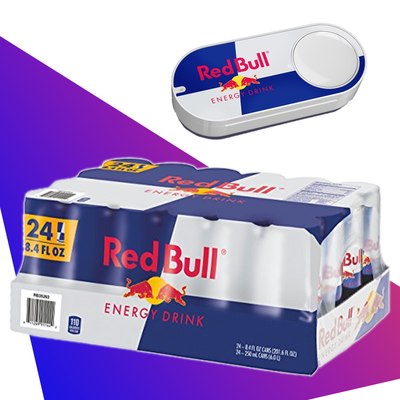
\includegraphics[scale = 0.7, center]{redbull-dash}
  \caption{The sold product}
\end{figure}
	%end of first chapter

	\chapter{Environment}		
In this section we give a precise definition of the customer classes and their features, cost functions and distribution probabilities on which the model is based.
		\section{Customer classes}
In the environment model we have three customer classes: C1, C2 and C3.
			\subsection{Class 1: the sportsman}
\lipsum[1]
			\subsection{Class 2: the programmer}
\lipsum[2]
			\subsection{Class 3: the retired man}
\lipsum[3]
		
	%end of second chapter

\chapter{Tasks}
\lipsum[4]
	%end of third chapter
	\chapter{References}
		\section{Links}

\begin{itemize}
	\item GitHub repository of the project: \url{https://github.com/tizianofucci/DIA2021AdvertisingAndPrincing}
\end{itemize}

\end{document}
